\newpage
\begin{center}
  \textbf{\large 1. ТЕОРЕТИЧЕСКАЯ ЧАСТЬ}
\end{center}
\refstepcounter{chapter}
\addcontentsline{toc}{chapter}{1. ТЕОРЕТИЧЕСКАЯ ЧАСТЬ}


Электростатические взаимодействия между мозаично распределенными на поверхности белка электрическими зарядами являются основным фактором, определяющим специфичность взаимодействий в~белковых комплексах~\cite{chrushev}. Поэтому при разработке оценочной функции для моделирования компонент в~виде <<твёрдых>> тел без конформационных изменений возможно опустить оценку ковалентных и~внутримолекулярных нековалетных взаимодействий. 

В~исследовании для описания межмолекулярных взаимодействий использовались общепринятые эмпирические парные потенциалы Леннард--Джонса и Кулона. Энергия растворителя вычислялась в~рамках модели неявного растворителя EEF1~\cite{eef1}. Процедура оценки энергии с~использованием оценочной функции разделяется на два этапа. 

На первом этапе формируется список взаимодействующих пар атомов в~зависимости от заданного радиуса сферы взаимодействия между атомами указанных компонент белкового комплекса. Для того, чтобы сформировать такой список возможно использовать прямой попарный перебор всех атомов с~определением евклидова расстояния. Очевидно, что такой подход очень затратен с~вычислительной точки зрения, поскольку каждый компонент комплекса состоит из нескольких тысяч атомов. Указанный этап оптимизируют с~использование различных структур данных. Описание выбранной структуры для оптимизации времени поиска атомов приведено в~разделе~1.2.

На втором этапе для каждой пары взаимодействующих атомов выполняется оценка энергии взаимодействия, а получившиеся значения суммируются формируя общую оценку взаимодействия для компонент белкового комплекса. Существуют различные подходы для оптимизации указанного этапа, однако они выходят за рамки выполняемой работы.

Разработанная оценочная функция состоит из трёх слагаемых:
\begin{equation}
	\displaystyle F_{s}=E_{v} + E_{c} + E_{s},
	\label{totalf}
\end{equation}
где~$E_{v}$ представляет собой оценку энергии, полученную с~помощью классического потенциала Леннард--Джонса~<<6--12>>, слагаемое~$E_{c}$ является оценкой энергии, полученной с~помощью потенциала Кулона, $E_{s}$ --~значение оценки энергии растворителя. В~следующем разделе для каждого компонента оценочной функции приведено описание с~указанием теоретических основ деталей применения. 

Поскольку разработка оценочной функции невозможна без учёта физических параметров атомов белка и~растворителя в~работе использовались данные широко распространённого силового поля CHARMM36~\cite{brooks}. Принципы применения~CHARMM и~описание используемых файлов силового поля для выполнения оценок представлены в~разделах ниже.

\addcontentsline{toc}{subsubsection}{Потенциалы оценочнной функции}

\section{Компоненты оценочной функции}

\subsection{Потенциал Кулона}

Электростатический потенциал Кулона описывает взаимодействие двух постоянных точечных зарядов и~определяется следующим образом
\begin{equation}
	E_{c}=\sum_{i,j}\left({\frac{1}{4 \pi \varepsilon_{r}}} \frac{q_{i}q_{j}}{d_{ij}} \left[ \frac{d^{2}_{ij}}{k^{2}} - \frac{2 d_{ij}}{k} + 1 \right]\right),
	\label{kp}
\end{equation}
где $d_{ij}$ -- евклидово расстояние между центрами атомов, $q_{i}$ и~$q_{j}$ --~фиксированные частичные атомные заряды в~рассматриваемой паре атомов, $\varepsilon_{r}$ --~диэлектрическая константа. Атомные заряды для каждого атома в~зависимости от типа получаются с~помощью программы PDB2PQR~\cite{pdb2pqr}. Вместо первой дроби при вычислениях используется константа, применяемая в~силовом поле CHARMM: $332.0716$~ккал${\cdot}$\AA${\cdot}e^{-2}/$моль. Последний множитель с~коэффициентом~$k=14$\AA \ определяет радиус сферы взаимодействия, для $d_{ij} > k$ вычисления не производятся.

Приведенный потенциал Кулона рассматривается не в~классическом виде. Как видно в~сумме~\ref{kp} используется дополнительный полиномиальный множитель --~квадратная функция, которая необходима для сглаживания значений потенциала при использовании коэффициента отсечения. Поскольку использование такого множителя применяется в~силовом поле~CHARMM принято решение использовать идентичный принцип вычисления потенциала. На рис.~\ref{vdw} представлены результаты вычисления потенциала Кулона без дополнительного множителя и~с~использованием дополнительным множителя.

\subsection{Потенциал Леннард-Джонса}

Потенциал Леннард-Джонса является моделью парного взаимодействия атомов, которая представляет собой математическую функцию описывающую силы притяжения и~отталкивания между атомами на основе их расстояния. Потенциал состоит из двух компонентов, которые позволяют смоделировать эффекты притяжения и~отталкивания.

Потенциал Леннард-Джонса <<6--12>> вычисляется по формуле
\begin{equation}
	\displaystyle E_{v}=\sum _{i,j}\left(\varepsilon_{ij}\left[\left({\frac {R_{ij}}{d_{ij}}}\right)^{12}-2\left({\frac {R_{ij}}{d_{ij}}}\right)^{6}\right]\right), \ R_{ij} = \frac{R_{i}}{2} + \frac{R_{j}}{2}, \ \varepsilon_{ij} = \sqrt{\varepsilon_{i} \varepsilon_{j}},
	\label{ld}
\end{equation}
где $d_{ij}$ -- евклидово расстояние между центрами атомов, $R_{i}$ и~$R_{i}$ -- расстояния, на которых значение потенциала становится равным нулю, $\varepsilon_{i}$ и~$\varepsilon_{j}$ -- глубины потенциальных ям. Указанные параметры получены из файла топологии для соответствующих типов атомов в рассматриваемой паре атомов с индексами $i$ и~$j$.

Необходимо отметить, что потенциал Леннард-Джонса в~классическом виде~\ref{ld} не используется в~силовом поле~CHARMM. Для описания сил Ван-дер-Ваальса используется двойной экспоненциальный потенциал~\cite{wu}. Он позволяет более точно оценить энергию, поскольку использует отдельные функции для оценки эффекта притяжения и~отталкивания, а~также отдельную процедуру для учета дальнодействующих взаимодействий. Отличия в~получаемых оценках продемонстрированы в~разделе 2.3.2. 

На рис.~\ref{vdw} приведены значения потенциала в~зависимости от расстояниям между двумя атомами: углерода ($\varepsilon=0.11, R/2 = 2$) и~водорода ($\varepsilon=0.031, R/2 = 1.25$).

\begin{figure}[h!]
	\captionsetup{justification=centering}
	\centering
	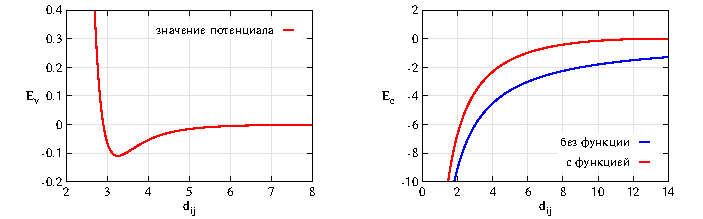
\includegraphics[width=1.0\linewidth]{images/vdwelec.pdf}
	\caption{Потенциал Леннард--Джонса. Потенциал Кулона с~применением дополнительного множителя и~без применения дополнительного множителя}
	\label{vdw}
\end{figure}

\subsection{Неявный растворитель}

Разрабатываемая оценочная функция в~дальнейшем планируется расширить для комплексов вида белок-ДНК. Белковые комплексы, которые могут связываться с~фрагментами~ДНК присутствуют в~большом количестве в~клетках организма человека~\cite{belov}. В~настоящей работе рассматриваются глобулярные водорастворимые белки --~класс белков, характеризующийся своей структурой и~растворимостью в~воде. Они имеют компактную, трехмерную структуру, свернутую в~форму шара или глобулы. Этот тип белков встречается в~цитоплазме клеток и~может выполнять разнообразные функции в~организме. 

Рассматриваемые в работе белковые комплексы проявляют свои нативные свойства лишь в~присутствии достаточного количества жидкой воды, которой в~цитоплазме приблизительно 80\%~\cite{water}. Из данных работы~\cite{wtwt} следует, что белки обладают гидратной оболочкой, которая представляет собой слой воды, окружающий макромолекулу. Следует отметить, что средняя плотность этой гидратной оболочки на 10\% выше, чем плотность объемной воды при аналогичных условиях. Таким образом, на поверхности белков образуется слой связанной воды, физические свойства которой отличаются от свойств воды в~объеме.

Взаимодействие с~молекулами воды существенно при образовании устойчивого комплекса, поэтому при оценке энергии взаимодействия с~помощью оценочной функции необходимо учитывать действие воды. Одним из самых простых способов моделирования действия водного раствора является неявный растворитель --~это математическая модель, используемая для моделирования взаимодействия биомолекул с~окружающим растворителем без явного учета молекул растворителя. Такой подход очень эффективен с~вычислительной точки зрения, поэтому при разработке было принято решение реализовать модель гауссовских гидратных оболочек EEF1~\cite{eef1}, которая используется для описания структуры гидратации белков. 

Гидратная оболочка атома --~слой молекул воды, которые окружают атом и~связаны с~ним посредством водородных связей. Гауссовские функции используются для моделирования гидратационной оболочки вокруг атомов белка, что позволяет более точно выполнить расчет энергии гидратации каждого отдельного атома. 

Следует отметить, что в силовом поле CHARMM присутствует возможность оценить энергию с~помощью неявного растворителя EFF1, но в~работе выполнена собственная реализация модели на основе статьи оригинальной~\cite{eef1} и~приведенной в~ней таблице значений для типов атомов. 

%Знание эффективной энергетической гиперповерхности биологических макромолекул в растворе имеет фундаментальное значение для понимания их свойств. Эффективная энергия (потенциал средней силы) для данной конформации макромолекулы представляет собой свободную энергию системы, состоящей из макромолекулы и растворителя, усредненную по всем степеням свободы растворителя при заданной температуре. Она состоит из внутримолекулярной энергии (энергия макромолекулы в вакууме) и энергии свободного растворения (свободная энергия переноса макромолекулы из газовой фазы в раствор). Общая свободная энергия системы макромолекула-растворитель в данной области гиперповерхности является суммой средней эффективной энергии и конфигурационной энтропии. В физиологических условиях обычно предполагается, что белки стабильны в окрестности глобального минимума (родной конформации), несмотря на большой прирост конфигурационной энтропии в денатурированном состоянии. Это называется "термодинамической гипотезой" стабильности белка, и имеющиеся данные свидетельствуют о ее справедливости для большинства малых однодоменных белков. Даже там, где эргодичность, кажется, нарушается, родное состояние должно соответствовать глубокому минимуму на эффективной энергетической гиперповерхности, который отделен от глобального минимума барьерами, слишком высокими для преодоления на экспериментальных временных шкалах. Теоретические прогнозы структуры белка из последовательности аминокислот и анализ механизма складывания требуют знания эффективной энергетической гиперповерхности и метода эффективного поиска конформационного пространства для определения расположения минимумов.

%Всеатомные силовые поля, используемые в молекулярной механике и динамике симуляций макромолекул, дают энгию белка в вакууме. Только введя явный растворитель и проведя симуляции, показывающие как макромолекулу, так и растворитель, можно учитывать эффекты соляции. Из результатов симуляций и теоретических соображений ясно, что эффективная гиперповерхность энергии, включающая растворитель, значительно отличается от внутримолекулярной гиперповерхности энергии. Хотя внутримолекулярная гиперповерхность энергии часто имеет глубокий минимум около нативной конформации, она может иметь другие равно глубокие или более глубокие минимумы в отдаленных областях пространства конформации. Это может возникнуть из-за ряда эффектов. Например, взаимодействия полярных-неполярных групп в газовой фазе энергетически выгодны так же, как и полярные-неполярные взаимодействия. Однако в воде полярно-неполярные взаимодействия эффективно отталкивают из-за высокого штрафа за десольватацию полярной группы. Кроме того, гидрофобная гидратация делает эффективные взаимействия между неполярными группами в воде сильнее, чем в газовой фазе. Таким образом, вода способствует стабилизации нативного состояния с зарытыми неполярными группами и помогает гарантировать его уникальность. Взаимодействия противоположных зарядов менее стабилизирующие в воде, чем в вакууме. Таким образом, проблемы, связанные с складыванием и стабильностью белков, не могут быть решены без учета соляции.

%Хотя за последние 40 лет был сделан значительный прогресс в статистической теории жидкостей, все еще отсутствуют простые и точные модели водной соляции. В настоящее время наиболее надежным методом учета соляции является симуляция белка в присутствии явных молекул воды. Однако этот подход связан с большими вычислительными затратами, и большая часть времени компьютера в таких симуляциях уходит на расчет взаимодействий растворителя-растворителя. Например в симуциях денатурации барназа система состояла из 1100 атомов белка и около 9000 атомов растворителя. Включение такого большого количества атомов растворителя ставит серьезные ограничения на тип проблем, которые можно изучать. Например, хотя динамику нативных состояний можно эффективно симулировать с помощью явных моделей растворителя, симуляции раскладки (и раскладанных состояний) на временных масштабах, необходимых для выборки достаточного количества различных начальных состояний для получения значимых сходимых результатов, пока что невозможны, за исключением, возможно, маленьких пептидов.

%Еще одним ограничем симуляций явной соляции является то, что разница свободной энергии не получается прямым способом. Например, точное моделирование воды в нативной и неправильно свернутой структурах не показывает, какая из них имеет наименьшую свободную энергию. Требуется особая симуляция, включающая обратимый переход от одной конформации к другой или выборка по зонтику, чтобы можно было рассчитать необходимые различия в свободной энергии. Такие симуляции были проведены главным образом для малых молекул, таких как бутан, дипептиды и другие маленькие пептиды. Недавно потенциал средней силы для маленького белка относительно радиуса инерции в качестве параметра порядка был рассчитан с явным растворителем; для этой симуляции потребовалось 450 часов процессорного времени на 64-узловом Т3Е-суперкомпьютере (эквивалент 4 месяцам на стандартной рабочей станции). Таким образом, использованте этого подхода для изучения деталей сложенных и раскладанных состояний ряда белков, а также многих других проблем текущего интереса, все еще невозможно. 

%Чтобы преодолеть ограничения вакуумных расчетов, с одной стороны, и явных симуляций растворителя, с другой, было разработано множество невных моделей соляции для белков, которые объединяют эмпирическое силовое поле для внутримолекулярных взаимодействий в вакууме с коррекцией сольвации. Последняя получается путем рассмотрения переноса всего белка или соответствующих составных групп из газовой фазы в воду. Очень простая модель использовала потенальную энергию CHARMM и коррекцию соляции на основе площади поверхности атома; были включены пять различных типов атомов. Та же модель соляции была объединена с силовым полем AMBER Шиффера. Фратернали и ван Гунстерен предложили еще более простую модель для использования в молекурной динамике (MD); эта модель также основана на доступных поверхностях и использует только два параметра - один для неполярных и один для полярных групп.

%Хотя вышеупомянутые модели оценивают эффект соляции в терминах площади поверхности, нет фундаментального теоретического обоснования для этого выбора. Модель, которая не использует площадь поверхности, - это модель гидратационной оболочки. Она предполагает, что свободная энергия гидратации группы возникает из первой гидратационной оболочки и пропорциональна объему гидратационной оболочки, доступной растворителю (т.е. не занятой другими атомами растворителя). Еще один тип модели соляции основан на контактах, которые каждая группа устанавливает с другими атомами растворителя. Чем больше контактов, тем меньше величина свобной энергии соляции группы, и контакты взвешиваются в соответствии с некоторой функцией их расстояния от группы. Эта модель похожа на подходы, использованные ранее Гибсоном, Шерагой и Левиттом. Физически, модель Колонна-Чезари-Сандера похожа на модели площади поверхности, но она намного быстрее в использовании, потому что подсчет количества контактов занимает значительно меньше времени, чем даже самые эффективные аналитические методы расчета площади поверности. Кроме того, аналитические производные свободной энергии соляции могут быть легко получены для оценки сил, необходимых для минимизации энергии и молекулярной динамики. Версия этой модели была параметризована на основе свободных энергий гидратации малых молекул. Для каждой группы назначается параметр соляции. Модель была объединена с полем сил GROMOS и использована в стохастической динамической симуляции инибита трипсина поджелудочной железы крупного рогатого скота (BPTI). Было обнаружено, что полученные структуры были разумными, хотя отклонение от кристалличкой структуры было немного больше, чем в симуляциях с явной водой. 

%Другой набор моделей сольватации рассматривает весь белок сразу и основан на континуальной электростатике и линеаризованном уравнении Пуассона-Больцмана. Поскольку численные решения уравнения Пуассона-Больцмана дороги, были предложены полуаналитические или аналитические приближения. Стилл ввел простое обобщение формулы Борна на многоатомные молекулы. Позднее обобщенное уравнение Борна было объединено с методом интегрированного поля для собственных энергий, что дало полностью аналитическую трактовку электростатических энергий и сил.38 Были сделаны приложения к ряду простых систем, и вполне вероятно, что этот подход будет использоваться более широко в будущем.

%\textbf{Описание модели.}

%Эффективная энергия $W(R^M)$ макромолекулы с координатами $R^M$ в решении может быть записана следующим образом

%\begin{equation}
	%W(R^M) = H_{intra}(R^M) + \Delta G^{slv}(R^M),
	%\label{ee}
%\end{equation}
%где 

%\begin{itemize}
	%\item $H_{intra}$ -- внутримакромолекулярная энергия
	%\item $\Delta G^{slv}$ -- свободная энергия растворителя
%\end{itemize}

%Чтобы получить данное уравнение \ref{ee}, единственное предположение состоит в том, что гамильтониан является сепарабельным; то есть это сумма терминов раствор-раствор, раствор-растворитель и растворитель-растворитель. Так обстоит дело с большинством эмпирических функций энергии, которые не включают поляризацию. Недавняя теоретическая работа по термодинамике сольватации показала, что свободная энергия сольватации $\Delta G^{slv}$ заданной конформации $R^M$ может быть записана как интеграл по окружающему пространству; то есть,

%\begin{equation}
	%\Delta G^{slv} = \int f(r)dr,
	%\label{fe}
%\end{equation}
%где $f(r)$ -- плотность свободной энергии сольватации в точке $r$. Она состоит из энергии расстворенного вещества-растворителя, энергии преобразования растворителя, энтропии раствора-растворителя и энтропии преобразования растворителя. Ожидается, что плотность свободной энергии растворителя сильно зависит от расстояния. Ее величина достигает максимума вблизи состояния раствора и стремится к нулю при отдалении от этого состояния. Когда две молекулы раствора приближаются друг к другу или изменяется конформация многоатомного раствора, сольватация каждой группы изменяется из-за двух эффектов: исключение растворителя из пространства, которое занято другими группами раствора, и изменение плотности ориентационного распределения растворителя в пространстве, которое не занято раствором. Для электростатических взаимодействий собственная энергия зарядов относится к первой категори, а диэлектрическое экранирование ко второй. В представленной модели упускается второй эффект для неполнярных групп, поскольку ожидается, что он будет незначительно малым, но он частично учитывается для полярных грпп за счет использования диэлетричской проницаемости, котороая зависит от расстояния. Предполагается, что для многоатомного раствора свободную энергию сольватации можно записать как сумму групп, то есть,

%\begin{equation}
	%\Delta G^{slv} = \sum_i \Delta G_i^{slv},
	%\label{fem}
%\end{equation}
%где $\Delta G_i^{slv}$ -- свободная энерегия сольватации группы $i$. Выражение \ref{fem} может быть формально получено путем рассмотрения энергии взаимодействия раствора и растворителя как суммы взаимодействия группы и растворителя и корреляционной функции раствора и растворителя как произведения корреляционных функций группы и растворителя. Принимая во внимание только эффект исключения растворителя, можно записать 

%\begin{equation}
	%\Delta G_i^{slv} = \Delta G_i^{ref} - \sum_j \int_{V_j} f_i(r) dr,
	%\label{femws}
%\end{equation}
%где $\Delta G_i^{ref}$ (эталонная свободная энергия сольватации) -- свободная энергия сольватации $i$ в молекуле, выбранной подходящим образом, в которой группа $i$ практически полностью подвергается воздействию растворителя. Интеграл в выражении находится по объему $V_j$ группы $j$, а суммирование происходит по всем группам $j$ вокруг $i$. Для упрощения вычислений интеграл по $f_i(r)$ заменяется произведением $f_i(r_{ij})V_j$, то есть

%\begin{equation}
%	\Delta G_i^{slv} = \Delta G_i^{ref} - \sum_{j \neq 1} f_i(r_{ij}) V_j,
%	\label{ufemws}
%\end{equation}
%где $r_{ij}$ -- расстояние между $i$ и $j$. Выражние \ref{ufemws} сообщает, что свободная энергия сольватации группы $i$ равна энергии в модельной системе $\Delta G_i^{ref}$ за исключением сольватации из-за присутствия окружающих групп. Предполагаемая плотность свободной энергии сольватации определяется функцией Гаусса.

%\begin{equation}
	%f_i(r) 4 \pi r^2 = \alpha_i exp(-x_i^2), x_i = \frac{r - R_i}{\lambda_i},
	%\label{gf}
%\end{equation}
%где $R_i$ -- ван дер Ваальсов радиус $i$, равный $\frac{1}{2}$ расстояния до энергетического минимума в потенциале Леннард-Джонса, $\lambda_i$ корреляционная длинна и $\alpha_i$ -- коэффициент пропорциональности, равный

%\begin{equation}
	%\alpha_i = \frac{2 \Delta G_i^{free}}{\sqrt{\pi \lambda_i}},
	%\label{kpr}
%\end{equation}
%где $\Delta G_i^{free}$ -- свободная энергия сольватации изолированной группы $i$; $\Delta G_i^{free}$ близка к $\Delta G_i^{ref}$, но не тождественно и определеяется эмпирически, требуя, чтобы свободная энергия сольватации глубоко лежащих групп равнялась нулю.


% TODO: потом убрать, если нисего отсюда не нужно
%Неявный растворитель -- это математическая модель, основанная на модели Гауссовских гидратных оболочек, которая используется для описания структуры гидратации белков и других макромолекул. Эта модель основана на предположении, что молекулы воды вблизи поверхности белка образовывают некоторую сферическую оболочку, в которой плотность молекул воды стремится к нулю. Разработчики использовали гауссовские функции, чтобы определить энергию гидратации каждого атома белка.

%Гидратная оболочка атома -- слой молекул воды, которые окружают атом и связаны с ним посредством водородных связей. То есть, гауссовские функции используются для моделирования гидратационной оболочки вокруг атомов белка, что позволяет более точно выполнить расчет энергии гидратации каждого отдельного атома.

%Модель Гауссовских гидратных оболочек предполагает, что размещение молекул воды в области гидратации с увеличением расстояния от белка может быть описано функцией Гаусса. Эта функция характеризуется средним значением и стандартным отклонением, которые определяют размеры и форму гидратной оболочки.

%Модель Гауссовских гидратных оболочек позволяет получить количественную оценку химических взаимодействий между белком и водой. В частности, эта модель используется для выявления ключевых аминокислотных остатков в белке, которые взаимодействуют с водой и играют важную роль в его структуре и функции.

%Более новые версии модели, такие как модель гидратации Майкросольвентной оболочки или модель Гижи-Шавитца, учитывают сильные динамические и корреляционные эффекты между молекулами воды и их взаимодействие с белком.

%Однако, важно понимать, что модель Гауссовских гидратных оболочек является лишь упрощенной моделью, которая не может учитывать полную динамику гидратации белка. Несмотря на это, она остается полезным инструментом для анализа структуры и функции белков в различных условиях.

%Формула неявного растворителя имеет вид:
%\[ E_s = \sum_i \Delta G_i + \sum_{i,j} \left( \frac{1}{2 \pi \sqrt{\pi}} \left[ -\Delta G_i e^{-\left( \tfrac{d_{ij} - {R_i}^{\textquotesingle}}{\lambda_i} \right)^2} - \Delta G_j e^{-\left( \tfrac{d_{ij} - {R_j}^{\textquotesingle}}{\lambda_j} \right)^2} \right] \right), \]
%где:
%\begin{itemize}
%	\item $d_{ij}$ -- евклидово расстояние между центрами атомов
%	\item $\lambda_i$ и $\lambda_j$ -- размеры гидратных оболочек атомов
%	\item ${R_i}^{\textquotesingle}$ и ${R_j}^{\textquotesingle}$ -- Ван-Дер-Ваальсовы радиусы атомов, которые соответствуют половине расстояния в потенциале Леннард-Джонса
%	\item $\Delta G_i$ и $\Delta G_j$ -- энергии гидратации в зависимости от типа атома
%\end{itemize}


Согласно модели EEF1 энергия растворителя $E_{s}$ вычисляется для комплекса по формуле:
\begin{equation}
	E_{s}=\sum_{i} \Delta G_{i} + \sum_{i,j}\left( \frac{1}{2\pi\sqrt{\pi}} \left[-\Delta G_{i} e^{-\left(\frac{d_{ij}-R_{i}^{\prime}}{\lambda_{i}}\right)^{2}}-\Delta G_{j}e^{-\left(\frac{d_{ij}-R_{j}^{\prime}}{\lambda_{j}}\right)^{2}}\right]\right),
	\label{eeffinal}
\end{equation}
где $d_{ij}$ --~евклидово расстояние между центрами атомов, $\lambda_{i}$ и~$\lambda_{j}$ --~размеры гидратных оболочек атомов. Параметры $R_{i}^{\prime}$ и~$R_{j}^{\prime}$ определяют Ван-дер-Ваальсовы радиусы атомов, которые соответствуют половине расстояния в~потенциале Леннард--Джонса, т.е. $R_{i}^{\prime}=R_{i}/2$, где $R_{i}$ --~параметр, используемый в~\ref{ld}. При вычислении первой суммы в~выражении~\ref{eeffinal} используются заранее вычисленные при температуре~$298.15$K значения полной энергии гидратации атомов~$\Delta G_{i}$. Перечисленные выше параметры представлены в~таблице~\cite{eef1} и~разбиты по группам для каждого типа атома. При реализации оценочной функции использовался принцип определения типов атомов, такой же, как и~в силовом поле CHARMM. 

\section{Структура данных k-d-дерево}

k-d-дерево -- это структура данных, которая позволяет эффективно хранить и~обрабатывать точки в~многомерном пространстве. Она используется для решения задач, связанных с~поиском ближайших соседей, поиском точек в~заданном диапазоне и кластеризацией данных.

k-d-дерево представляет собой бинарное дерево, в~котором каждый узел соответствует гиперплоскости, разбивающей пространство на две части. Каждый узел содержит точку из множества, которое нужно организовать, а~также указатели на двух потомков -- левого и~правого.

При поиске ближайших соседей или точек в заданном диапазоне, происходит спуск по дереву, выбирая тот узел, который содержит искомую точку. Затем происходит проверка точек в~этом поддереве и, если они удовлетворяют условию поиска, то происходит их добавление в~результат. Если же поддерево не содержит искомую точку, происходит переход к~следующему поддереву, пока не будет найдена нужная точка или не произведен обход всех поддеревьев.

Для построения k-d-дерева необходимо выбрать гиперплоскость, которая будет разбивать пространство на две части. Это можно сделать различными способами, например, выбрать гиперплоскость, которая проходит через среднюю точку множеств, или выбрать гиперплоскость, которая и~в~разных поддеревьях.

Структура данных k-d-дерево имеет ряд преимуществ перед другими структурами данных, такими как массивы или хэш-таблицы. Оно позволяет эффективно хранить и~обрабатывать большие объемы данных, а~также быстро выполнять операции поиска, что важно для поставленной задачи. Применение k-d-дерева является классическим решением задачи оптимизации поиска взаимодействующих атомов и~применяется, в~том числе, в~пакете~Rosetta.

\section{Силовое поле CHARMM}

Разработанная оценочная функция использует текстовый файл топологии, который представляет собой набор параметров и~топологических данных, используемых для моделирования и~симуляции белков с~использованием программного пакета CHARMM. Файл $par\_all36m\_prot.prm$ свободно распространяется и~требуется для разработанной в~настоящей работе оценочной функции, поскольку содержит необходимые параметры для атомов при вычислении оценки потенциалом Леннард-Джонса.

В этом файле содержится информация о~параметрах и~топологии для атомов, взаимодействий и~других особенностей белковой структуры. Несмотря на то, что он также содержит информацию о~зарядах атомов, которые получены из экспериментальных данных или рассчитаны с использованием квантово-химических методов, для разработанной оценочной функции информация была получена с~использованием программы pdb2pqr~\cite{pdb2pqr}.

Несмотря на то, что CHARMM открыто распространяется его использование для выполнения оценок затруднительно с~вычислительной точки зрения. Применение CHARMM требует преобразования исходного файла~PDB во внутреннее представление пакета, которое включает в~себя несколько шагов. На рис.~\ref{charmm} взятого из~\cite{brooks} представлен путь, который необходимо пройти исходному файлу PDB для получения энергии взаимодействия. Использовать пакет CHARMM напрямую из разрабатываемой в~рамках научно-исследовательской работы библиотеки реализованной на~C++ затруднительно. Указанные недостатки применения CHARMM легли в~основу постановки целей текущей работы.


\begin{figure}[h!]
\begin{center}
	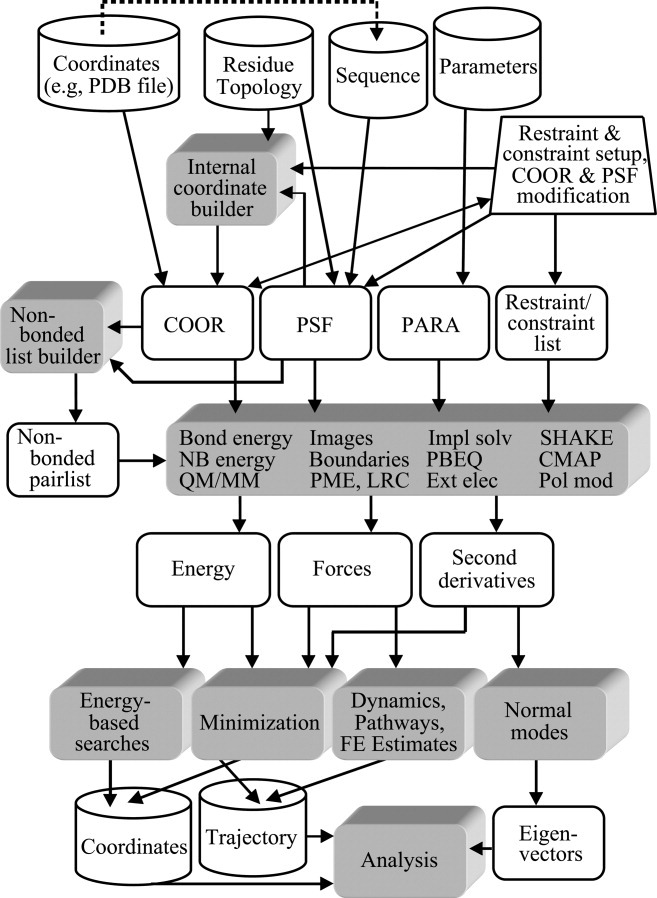
\includegraphics[width=0.5\textwidth]{images/charmm.jpg}
	\caption{Общая схема проекта CHARMM}
    \label{charmm}
\end{center}
\end{figure}


%\section{Описание входных данных}


\section{Форматы данных PDB (Protein Data Bank) и PQR}

Все рассматриваемые белковые комплексы изначально имеют формат PDB. Архив PDB представляет собой хранилище атомных координат и~другой информации, описывающей белки и~другие важные биологические макромолекулы. Структурные биологи используют такие методы, как рентгеновская кристаллография, ЯМР-спектроскопия и криоэлектронная микроскопия, чтобы определить положение каждого атома относительно друг друга в~молекуле. 

Первичная информация, хранящаяся в архиве PDB, состоит из файлов координат биологических молекул. В этих файлах перечислены атомы в каждом белке и~их трехмерное расположение в~пространстве. Эти файлы доступны в~нескольких форматах (PDB, mmCIF, XML). Типичный файл в формате PDB включает в~себя большой раздел <<заголовка>>, текста, в~котором резюмируется белок, информация о~цитировании и~детали структурного решения, за которым следует последовательность и длинный список атомов и~их координат. Архив также содержит экспериментальные наблюдения, которые используются для определения этих атомных координат.

%Визуализация структур
%Возможно просматривать файлы PDB напрямую с помощью текстового редактора, часто наиболее полезно использовать программу просмотра или визуализации для их просмотра. Онлайн-инструменты, такие как на веб-сайте RCSB PDB, позволяют искать и изучать информацию под заголовком PDB, включая информацию об экспериментальных методах, химии и биологии белка.

%Потенциальные проблемы
%При изучении архива PDB может возникуть ряд проблем. Например, многие структуры, особенно определяемые кристаллографией, включают информацию только о части функциональной биологической сборки. Кроме того, во многих записях PDB отсутствуют части молекулы, которые не наблюдались в эксперименте. К ним относятся структуры, включающие только положения альфа-углерода, структуры с отсутствующими петлями, структуры отдельных доменов или субъединиц более крупной молекулы. Кроме того, в большинстве записей кристаллографической структуры отсутствует информация об атомах водорода.

%Центральным хранилищем данных о структуре биологических макромолекул является Protein Data Bank, доступный по адресу rcsb.org.

Уникальным идентификатором каждой структуры в~Protein Data Bank является PDB~ID. Данный идентификатор состоит из четырех символов, первый из которых, как правило, цифра; буквы в~PDB ID принято писать заглавными, хотя большинство программ в~данном случае не~чувствительны к регистру символов. 

В файле данного формата каждая колонка обладает строго определенную длину и содержит определенную информацию: 1-6 -- имя записи; 7-11 -- серийный номер атома; 13-16 -- имя атома; 17 -- альтернативное имя атома; 18-20 -- имя остатка; 22 -- идентификатор цепи; 23-26 -- номер остатка; 27 -- код для вставки остатков; 31-38 -- координата X атома; 39-46 -- координата Y атома; 47-54 -- координата Z атома; 55-60 -- вместимость; 61-66 -- температура; 77-78 -- символ элемента; 79-80 -- заряд атома.

Любые электростатические расчеты начинаются с~определения структуры молекулы, параметров заряда и~размера составляющих её атомов и~свойств растворителя. APBS предоставляет программную утилиту pdb2pqr~\cite{pdb2pqr}, которая позволяет преобразовать входной файл в~формате PDB в~формат~PQR.

Формат PQR (Protein Data Bank PQR format) является модификацией формата PDB (Protein Data Bank format), используемого для хранения информации о структуре биомолекул, таких как белки, нуклеиновые кислоты и другие макромолекулы. PQR расшифровывается как <<PDB with Charges and Radii>> (PDB с~зарядами и радиусами) и содержит дополнительные сведения о зарядах и радиусах атомов в~молекуле.

Основное отличие формата PQR от PDB заключается в~наличии дополнительной информации о~зарядах и~радиусах атомов. В~PQR файле каждому атому присваивается заряд (обычно расчетный или эмпирический) и~радиус, которые важны для проведения различных анализов и моделирования, включая расчеты электростатических взаимодействий и~проницаемости растворителя. Следует отметить, что при преобразовании можно явно указать водородный показатель~pH раствора.


%\subsection{Формат данных PQR}

%Надежные модели электростатических взаимодействий важны для понимания событий раннего молекулярного распознавания, где доминируют дальнодействующие межмолекулярные взаимодействия и эффекты сольватации на биомолекулярные процессы. В то время как явные электростатические модели, которые рассматривают растворенное вещество и растворитель в атомарных деталях, являются общими, эти подходы обычно требуют тщательного уравновешивания и отбора проб для сведения интересующих свойств в интересующий статистический ансамбль. Континуальные подходы, которые интегрируют важные, но в значительной степени неинтересные степени свободы, жертвуют численной точностью в пользу надежной, но качественной точности и эффективности, устраняя необходимость отбора проб и уравновешивания, связанную с явными моделями растворов и растворителей.

%Хотя существует выбор между несколькими моделями неявной сольватации, одна из самых популярных моделей неявной растворимости для биомолекул основана на уравнении Пуассона–Больцмана (ПБ). Уравнение ПБ обеспечивает глобальное решение для электростатического потенциала $\phi$ внутри и вокруг биомолекулы путем решения уравнения в частных производных

%\begin{equation}
%	\Delta \epsilon \Delta \phi - \sum_i^M c_i q_i e^{-\beta(q_i \phi + V_i)} = \rho
%	\label{pde}
%\end{equation}

%Растворитель описывается объемной диэлектрической проницаемостью растворителя $\varepsilon_s$ и свойствами подвижных ионов $i = 1, ..., M$ описываемыми их зарядами $q_i$, концентрациями $c_i$ и стерическим потенциалом взаимодействия ионов с раствором $V_i$. Биомолекулярная структура включена в уравнение через $V_i$, функцию диэлектрического коэффициента и функцию распределения заряда $\rho$. Диэлектрическая проницаемость $\epsilon$ часто устанавливается равной постоянному значению $\varepsilon_{min}$ внутри молекулы и резко меняется на молекулярной границе до значения $\varepsilon_s$, которое описывает объем растворителя. Форма границы определяется размером и расположением атомов раствора, а также специфическими для модели параметрами, такими как характерный размер молекулы растворителя. Распределение заряда $\rho$ обычно представляет собой сумму дельта-распределений Дирака, расположенных в центрах атомов. Наконец, $\beta = {(5 \kappa T)}^{-1}$ — обратная тепловая энергия, где $\kappa$ -- постоянная Больцмана, а $T$ — температура. Потенциал $\phi$ может использоваться в различных приложениях, включая визуализацию, другие структурные анализы, моделирование диффузии и ряд других расчетов, требующих глобальных электростатических свойств. Теория ПБ является приближенной и, как следствие, имеет несколько хорошо известных ограничений, которые могут повлиять на ее точность, особенно для сильно заряженных систем или высоких концентраций солей. Несмотря на эти ограничения, методы ПБ по-прежнему очень важны и популярны для биомолекулярного структурного анализа, моделирования и симуляции.

%Было разработано несколько пакетов программного обеспечения, которые решают уравнения Пуассона-Больцмана для оценки энергий, потенциалов и других свойств сольватации. Наиболее значимые (на основе пользовательской базы и цитирований) из них: CHARMM, AMBER, DelPhi, Jaguar, Zap, MIBPB и APBS. Тем не менее, APBS и связанный программный пакет PDB2PQR служат большому сообществу, насчитывающему около 27 000 пользователей, путем создания веб-серверов, связанных с веб-сайтом APBS, которые поддерживают подготовку биомолекулярных структур и быстрое решение методом конечных разностей. уравнения Пуассона–Больцмана, которые дополнены набором инструментов анализа. Еще более широкий набор функций и более гибкая конфигурация доступны, когда APBS и PDB2PQR запускаются из командной строки на платформах Linux, Mac и Windows, и которые можно запускать локально или через веб-службы, предоставляемую разработанным NBCR набором инструментов Opal. Этот инструментарий позволяет переносить вычислительную нагрузку для научных приложений с интенсивным использованием процессора на удаленные вычислительные ресурсы, такие как ресурсы, предоставляемые Национальным ресурсом биомедицинских вычислений (NCBR). Наконец, APBS может работать с другими программами молекулярного моделирования, такими как AMBER, CHARMM, NAMD, Rosetta и TINKER. Общая поддержка интеграции APBS со сторонними программами обеспечивается библиотекой iAPBS.



